\documentclass[fleqn,10pt,lineno]{manuscript}
%%\usepackage{setspace}
%%\doublespacing
\usepackage{soul, hyperref}
\usepackage[utf8]{inputenc}

\newcommand{\beginsupplement}{%
        \setcounter{table}{0}
        \renewcommand{\thetable}{S\arabic{table}}%
        \setcounter{figure}{0}
        \renewcommand{\thefigure}{S\arabic{figure}}%
     }

\title{A Structural and Functional Bioinformatics Study of QTY-designed Retinylidene Proteins}

\author[1]{Siqi Pan}
\author[2]{Shuguang Zhang}
\affil[1]{Shanghai World Foreign Language Academy, 400 Baihua Street, Shanghai 200233, China}
\affil[2]{Lab of Molecular Architecture, Media Lab, Massachusetts Institute of Technology, 77 Massachusetts Avenue, Cambridge, MA 02139, USA}

\corrauthor[2]{Shuguang Zhang}{Shuguang@MIT.EDU}

\keywords{hydrophobic to hydrophilic conversion; membrane proteins; protein design; QTY code; water-soluble retinylidene proteins; water-soluble opsins; activation of QTY variants of rhodopsin}
\begin{abstract}

This study investigates the QTY design of 9 human and 3 microbial retinylidene proteins ... [TO BE WRITTEN]



\end{abstract}

\begin{document}

\flushbottom
\maketitle
\thispagestyle{empty}

\section*{Introduction}

Retinylidene proteins are photochemically reactive proteins that are bound to or can bind to retinal (vitamin A aldehyde) as their chromophore \citep{Spudich_2000}. We will use the term ``opsin'' interchangeably with ``retinylidene protein'', despite the fact that ``opsin'' sometimes refers specifically to the chromophore-free apoprotein. Retinylidene proteins are divided into two groups, animal opsins and microbial opsins, which are evolutionarily distinct but share common characteristics such as having 7 transmembrane (TM) domains and a retinal binding lysine residue \citep{Yee_2013, Spudich_2000}. In this study, we will consider 9 animal opsins and 3 microbial opsins. 

\textbf{Animal opsins} are a type of class A GPCR (G-protein coupled receptor), which are characterized by 7 transmembrane domains, the NPxxY motif, and activation of G-proteins through the outward movement of TM6. \citep{Sakmar_2002, Nordstrom_2011, Zhou_2019}. Almost all animal opsins include a lysine residue that forms a Schiff base link with the retinal \citep{Bownds_1967, Guhmann_2022}. When retinal absorbs a photon, it isomerizes, usually changing from 11-cis to all-trans. The subsequent conformational changes of the protein are well studied using bovine rhodopsin, which changes from dark state to BATHO state, then LUMI, META I, and META II \citep{Okada_2001, Smith_2010}. Proton transfer plays a major role in this process \citep{Mahalingam_2008}. During this process, TM6 is characteristically moved outward, activating the G-protein. 

In this study, we selected 9 opsins expressed in the human nervous system: OPN1MW (\href{https://www.uniprot.org/uniprotkb/P04001/entry}{P04001}), OPN1LW (\href{https://www.uniprot.org/uniprotkb/P04000/entry}{P04001}), OPN1SW (\href{https://www.uniprot.org/uniprotkb/P03999/entry}{P03999}), OPN2 (\href{https://www.uniprot.org/uniprotkb/P08100/entry}{P04001}), OPN3 (\href{https://www.uniprot.org/uniprotkb/Q9H1Y3/entry}{Q9H1Y3}), OPN4 (\href{https://www.uniprot.org/uniprotkb/Q9UHM6/entry}{Q9UHM6}), OPN5 (\href{https://www.uniprot.org/uniprotkb/Q6U736/entry}{Q6U736}), RGR (\href{https://www.uniprot.org/uniprotkb/P47804/entry}{P47804}) and RRH (\href{https://www.uniprot.org/uniprotkb/O14718/entry}{O14718}). They belong to several evolutionarily distinct families of animal opsins \citep{Terakita_2005, Shichida_2009}. 

\textbf{OPN1MW} (Medium-Wave-sensitive Opsin 1), \textbf{OPN1LW} (Long-Wave-sensitive Opsin 1) and \textbf{OPN1SW} (Short-Wave-sensitive Opsin 1) are expressed in retinal cone photoreceptors and are responsible for color vision \citep{Bowmaker_1980}. Certain variants of OPN1MW, OPN1LW and OPN1SW respectively cause deutanopia, protanopia, and tritanopia, which are different types of color blindness \citep{Ueyama_2002, Baraas_2012}. The absence of both functional OPN1MW and OPN1LW causes blue cone monochromacy, an X-linked congenital cone dysfunction syndrome \citep{Wissinger_2022}, and cone dystrophy 5, an X-linked cone dystrophy \citep{Gardner_2010}. 

\textbf{OPN2} (Opsin 2), also known as rhodopsin, is expressed in retinal rod photoreceptors and is responsible for vision at low light intensity \citep{Hubbard_1958}. Certain variants lead to autosomal recessive or autosomal dominant retinitis pigmentosa \citep{Fanelli_2021}. Other variants also lead to congenital stationary night blindness \citep{Fanelli_2021}. OPN2 is a representative animal opsin, one of the earliest studied \citep{Hubbard_1958}. In fact, bovine OPN2 is the first opsin to be sequenced \citep{Nathans_1984} as well as the first GPCR whose crystal structure was resolved experimentally \citep{Palczeski_2000}. Many studies on the functional mechanisms of animal opsins also focus on OPN2 \citep{Park_2008, Scheerer_2008, Kimata_2016}. Consequently, we also choose OPN2 to conduct a functional analysis in this study, in order to further explore the effectiveness of the QTY design of retinylidene proteins. 

\textbf{OPN3} (Opsin 3), also known as encephalopsin or panopsin, is activated by blue and ultraviolet A light. It is expressed in the brain \citep{Blackshaw_1999}. It is also expressed in melanocytes and keratinocytes in the skin and regulates functions such as melanogenesis, cell differentiation, and glucose uptake \citep{Koyanagi_2013, Olinski_2020}. 

\textbf{OPN4} (Opsin 4), also known as melanopsin, is expressed in ipRGC (intrinsically photosensitive Retinal Ganglion Cells) in the ganglion cell layer in the retina \citep{Provencio_1998}. It is responsible for pupillary reflex, photoentrainment, optokinetic visual tracking response, and other non-image-forming responses to light \citep{Berson_2002, Gooley_2003}. 

\textbf{OPN5} (Opsin 5), also known as neuropsin, is activated by blue and ultraviolet A light \citep{Tarttelin_2003, Yamashita_2010}. It is expressed in the retina and contributes to the regulation of light-dependent vascular development \citep{Nguyen_2019} and photoentrainment in the cornea and retina \citep{Buhr_2015}. 

\textbf{RGR} (RPE-retinal GPCR) is expressed in RPE (Retinal Pigmented Epithelium) and M\"uller cells in the retina \citep{Shen_1994}. Unlike the aforementioned human opsins, RGR preferentially binds all-trans-retinal and may catalyze its isomerization into 11-cis-retinal via a retinochrome-like mechanism \citep{Radu_2008}. It plays a role in the light-dependent synthesis of visual chromophore \citep{Radu_2008}.

\textbf{RRH} (RPE-derived Rhodopsin Homolog), also known as peropsin, is localized in the microvilli of RPE cells that surround photoreceptor outer segments \citep{Sun_1997}. It is another protein that preferentially binds to all-trans-retinal \citep{Cook_2017}. 

\textbf{Bacterial opsins} are transmembrane ion pumps or channels \citep{Findlay_1986, Zhang_2011}. They are also 7TM, though this is due to convergent evolution rather than homology \citep{Yee_2013}. The isomerization of retinal is usually from all-trans to 13-cis, different from that in animal opsins \citep{Findlay_1986, Spudich_2000}. In addition, bacterial opsins often form oligomers to carry out their functions \citep{Taguchi_2023, Gmelin_2007, Shan_2024}.

In this study, we selected 3 bacterial opsins: BACR (\href{https://www.uniprot.org/uniprotkb/P02945/entry}{P02945}), BACH (\href{https://www.uniprot.org/uniprotkb/B0R2U4/entry}{B0R2U4}), ChR2 (\href{https://www.uniprot.org/uniprotkb/Q8RUT8/entry}{Q8RUT8}). 

\textbf{BACR} (Bacteriorhodopsin) is a light-driven proton pump \citep{Oesterhelt_1971}. \textbf{BACH} (Halorhodopsin) is a light-driven chloride pump activated by yellow light \citep{Schobert_1982}. \textbf{ChR2} (Channelrhodopsin 2) is a light-activated sodium channel activated by blue light \citep{Nagel_2003}. BACH and ChR2 are among the first optogenetic tools \citep{Zhang_2007, Han_2007}. BACH is used for inhibition, while ChR2 is used for excitation. 

We have asked if retinylidene proteins could be redesigned to be more soluble. Retinylidene proteins are all integral membrane proteins with seven transmembrane alpha helices embedded in a lipid bilayer. Because of the hydrophobic properties of the transmembrane domains, they are not water-soluble without the aid of detergents. 

Bacteriorhodopsin has been the subject of several protein-solubilizing studies, though with limited success \citep{Sirokman_1993, Gibas_1997, Mitra_2002}. Recently, researchers leveraged a neural network, SolubleMPNN, which was built upon ProteinMPNN, to engineer soluble variants of bacteriorhodopsin while maintaining its ligand-binding ability and light-sensing function \citep{Nikolaev_2024}.

Instead of taking a computational approach, we applied the QTY (Glutamine, Threonine, Tyrosine) code to systematically engineer water-soluble analogs with reduced hydrophobicity in membrane proteins. There are structural similarities between hydrophobic and polar amino acids: leucine (L) vs. glutamine (Q); isoleucine (I) / valine (V) vs. threonine (T); and phenylalanine (F) vs. tyrosine (Y), as can be observed on high-resolution electron density maps \citep{Zhang_2018, Zhang_2022, Tegler_2020}. This justifies the replacement of hydrophobic amino acids with polar ones. We initially applied the QTY code to design several detergent-free chemokines receptors, all of which retained structural thermal stability and native ligand-binding activities and enzymatic activities despite substantial changes to the transmembrane domain \citep{Zhang_2018, Tegler_2020}. We have also applied the QTY code to design water-soluble GPCRs, including chemokine receptors \citep{Zhang_2018, Qing_2019, Tegler_2020, Skuhersky_2021}, cytokine receptors \citep{Hao_2020}, and olfactory receptors \citep{Skuhersky_2021, Johnsson_2025}. 

AlphaFold2 was released by Google DeepMind in July 2021 \citep{Jumper_2021}. It greatly facilitated the study of QTY-designed protein variants. Subsequently, AlphaFold3 was released in May 2024, featuring improved architecture and improved efficiency \citep{Abramson_2024}. Furthermore, AlphaFold3 enabled the accurate prediction of complexes of multiple proteins, as well as complexes with nucleic acids and certain small molecules. QTY studies have made use of these new features \citep{Chen_2025, Johnsson_2025}. 

GROMACS is a molecular dynamics (MD) simulation program released in 1995 \citep{Berendsen_1995}. Its 5.0 version was released in 2015 \citep{Abraham_2015}. GROMACS enables an efficient and realistic simulation of biomolecular systems, and has been used to investigate the structural and functional properties of QTY-designed protein variants in various studies \citep{Karagol_2024, Li_Tang_2024, Smorodina_2024, Li_Wang_2024, Johnsson_2025}. 

In this paper, we apply the QTY code to redesign 9 human opsins and 3 microbial opsins. We provide the superpositions of the AlphaFold3-predicted hydrophobic native proteins and their water-soluble QTY variants, and experimentally-determined structures when available. We also provide a comparison of the surface hydrophobicity of the variants. Furthermore, we run MD simulations of native and QTY-designed OPN2 and analyze their response to the 11-cis to all-trans isomerization of the retinal chromophore. 

\section*{Results and Discussion}

\subsection*{The QTY code}

Discuss the QTY code. 

\subsection*{Retinylidene proteins sequence alignments and other characteristics}

Describe and discuss Table~\ref{tb:characteristics} (native and QTY protein characteristics) // NOTE: the binding of retinal is posterior to folding, so it is safe to say that we predicted chromophore-free form (i.e. folding does not rely on retinal). 

\subsection*{Superpositions of AlphaFold3-predicted native human opsins, their water-soluble QTY variants, and experimentally determined structures}

Describe and discuss Fig.~\ref{fig:humansup} (AF3 native - AF3 QTY - experimental superpositions of human opsins). 

\subsection*{Pairwise superpositions among AlphaFold3-predicted native human opsins and among their water-soluble QTY variants}

Describe and discuss Fig.~\ref{fig:pairwise} (pairwise superpositions of human opsins) // NOTE: the QTY pairwise superpositions roughly maintains the trends in the native superpositions. 

\subsection*{Superpositions of AlphaFold3-predicted native microbial opsins, their water-soluble QTY variants, and experimentally determined structures}

Describe and discuss Fig.~\ref{fig:microbialsup} (AF3 native - AF3 QTY - experimental superimpositions of microbial opsins) // NOTE: comment specifically on the formation of dimers and trimers. 

\subsection*{Analysis of the hydrophobic surface of native retinylidene proteins and their water-soluble QTY variants}

Describe and discuss Fig.~\ref{fig:hydrophobicity} (surface hydrophobicity). 

\subsection*{AlphaFold3 predictions}

Discuss the role of AlphaFold3 predictions. 

\subsection*{Simulation of 11-cis to all-trans isomerization of retinal in native OPN2 and its QTY variant}

Describe, explain, discuss MD simulation results. // NOTE: there were no changes to the NPxxY motif or retinal-binding Lys; "The ionic environment of the RSB, defined by the residues of the binding pocket, dictates the spectral and kinetic characteristics of each individual protein." \citep{Fenno_2011}, so QTY variant may have different absorption peak. 

MD Results
* different states - binding pocket residues + ligand orientation
* bond length, angle, dihedral, non-bonded interaction lengths graph
* by-helix rmsd
* by-residue IE
* hbond
* overall rmsd, gyrate, rmsf, IE

\subsection*{Future scopes and potential applications}

Future scopes and potential applications. 

\subsection*{Conclusion}

Conclusion

\section*{Methods}

\subsection*{QTY design, protein sequence alignment and other characteristics}

The native protein sequences for OPN1MW, OPN1LW, OPN1SW, OPN2, OPN3, OPN4, OPN5, RGR, RRH, BACR, BACH, and ChR2 were obtained from UniProt (\url{https://www.uniprot.org}). The sequence for ChR2 was truncated according to the experimental structure in RCSB PDB (\href{https://www.rcsb.org/structure/8ZAN}{8ZAN}). The QTY designs were performed through the Protein Solubilizing Server (\url{https://pss.sjtu.edu.cn/}) \citep{Tao_2022}. For ChR2, the secondary structure was provided to the server in SS3 format according to the RCSB PDB structure. 

\subsection*{AlphaFold3 predictions}

We predicted the structures of native proteins and their QTY variants using the AlphaFold3 website (\url{https://alphafoldserver.com}) \citep{Abramson_2024}. For microbial opsins, the dimers and trimers had identical subunits, i.e., they were homodimers and homotrimers. In AlphaFold3, this was achieved by altering the number of protein copies. 

\subsection*{Structure superpositions}

PDB files for native protein structures determined experimentally by X-ray diffraction or electron microscopy were taken from RCSB PDB: OPN2 (\href{https://www.rcsb.org/structure/5W0P}{5W0P}), BACR (\href{https://www.rcsb.org/structure/7XJC}{7XJC}), BACH (\href{https://www.rcsb.org/structure/2JAF}{2JAF}), ChR2 (\href{https://www.rcsb.org/structure/8ZAN}{8ZAN}). The AlphaFold3-predicted native and QTY variants were taken directly from the most probable predicted structure. Superpositions were performed via the command ``super'' in PyMOL (\url{https://pymol.org}). We remove unstructured loops at the N and C terminals for the sake of clarity. 

\subsection*{Structure visualization}

We used PyMOL (\url{https://pymol.org}) to superpose the native predicted protein structures, their QTY variants, and the experimental structures for the proteins where these existed. We then used UCSF ChimeraX (\url{https://www.cgl.ucsf.edu/chimerax/}) to render each protein model with hydrophobicity patches.  

\subsection*{Molecular dynamics simulations}

All MD simulations and analyses were executed on a desktop computer with Intel Xeon Platinum 8352V Processor, 256 GB RAM, and 2 NVIDIA GPU (GeForce RTX 4090) with 24 GB VRAM each. All MD simulations were conducted using GROMACS 2024.5 \citep{Abraham_2015} with the CHARMM36m all-atom force field \citep{Huang_2017}. Data for retinal were obtained from NAMD Wiki (\url{https://www.ks.uiuc.edu/Research/namd/wiki/index.cgi?RetinalTop} for topology and \url{https://www.ks.uiuc.edu/Research/namd/wiki/index.cgi?RetinalPar} for parameters) and manually integrated into the protein file. Initial structures, configuration files, and command-line codes for the simulations are publicly available at... [ONLINE DATABASE TO BE PREPARED]. 

Regarding native OPN2, the membrane protein system was constructed using the web-based membrane builder CHARMM-GUI and was downloaded in GROMACS format \citep{Jo_2008, Wu_2014, Lee_2016}. The protein was centered in a rectangular box. The generated membrane models consisted of 40\% POPC, 40\% POPE, 10\% POPS, and 10\% cholesterol, which simulate a rod photoreceptor disk membrane \citep{Albert_2005}. The system was solvated in TIP3P water with 150 mM NaCl. 11-cis-retinal was manually added to the protein files. LINCS constraints were used for constraints, and Verlet integrator was used. Electrostatics was handled with Particle Mesh Ewald (PME), with both Coulomb and van der Waals interaction cutoffs set at 1.2 nm. The energy of the system was minimized using the steepest descent until the maximum forces converged below 1000 kJ/mol/nm. The standard six-step CHARMM-GUI NP$\gamma$T equilibration protocol \citep{Jo_2008} was used, with two 125-ps NVT equilibration simulations, and one 125-ps and three 500-ps NP$\gamma$T equilibration simulations. Temperature and pressure were maintained at 303.15 K and 1.0 bar, respectively, using the V-rescale thermostat and C-rescale barostat with surface-tension coupling. Following equilibration, a 10-ns production MD simulation was run. The retinal molecule was then manually switched to the all-trans state by rotating C13 to C15 and bonded hydrogen and methyl groups by 180 degrees around the C11-C12 bond. Energy minimization and equilibration were repeated exactly as before, and then a 200-ns production MD simulation was run. 

Regarding QTY-designed OPN2, the system was constructed directly using GROMACS. The protein was centered in a rectangular box with dimensions equivalent to those of native OPN2. The equilibration involved a sequence of simulations: a 250-ps NVT equilibration, followed by 125-ps and 1500-ps NPT equilibrations, totaling an equilibration duration that matches that of the natural OPN2. All other configurations and parameters are identical to those of the original OPN2.

[ANALYSIS METHODS OF MD SIMULATION RESULTS, TO BE ADDED.]

\section*{Supplementary Material}

The supplementary material can be found at... [TO BE ADDED]

\section*{Data Availability Statement} 

The data for... can be found at... [ONLINE DATABASE TO BE PREPARED]

\section*{Author contributions}

Conceptualization: S.P., S.Z.; Formal analysis: S.P.; Investigation: Methodology: S.P.; Validation: S.P.; Data curation: S.P.; Writing—original draft preparation: S.P., S.Z.; Review and editing: S.P., S.Z. 

\section*{Financial Support}

There is no financial support for this digital bioinformatics study. We only used free tools that are publicly available. 

\section*{Acknowledgments}

Thanks to... for... [TO BE ADDED]


\section*{Competing Interests}

Massachusetts Institute of Technology (MIT) filed several patent applications for the QTY code for GPCRs excluding the human opsins. OH2Laboratories licensed the technology from MIT to work on water-soluble GPCR variants. S.Z. is an inventor of the QTY code and has a minor equity in OH2Laboratories. S.Z. is a Scientific Advisor and has minor shares for a startup RealNose to develop a sensing device based on olfactory receptors. S.Z. founded a startup 511 Therapeutics to generate therapeutic monoclonal antibodies against solute carrier transporters to treat pancreatic cancer. S.Z. has majority equity in 511 Therapeutics. All other authors have no competing interests.


\section*{Ethics Statement}

All methods were carried out in accordance with relevant guidelines and regulations. All experimental protocols were approved by a named institutional and licensing committee. Neither human biological samples nor human subjects were used in the study. This is a completely digital structural bioinformatic study using the publicly available AlphaFold3 machine learning program and GROMACS molecular dynamics simulation program.


\bibliography{references}

\begin{table}[htbp]
	\centering
	\caption{Protein characteristics}
	\label{tb:characteristics}
	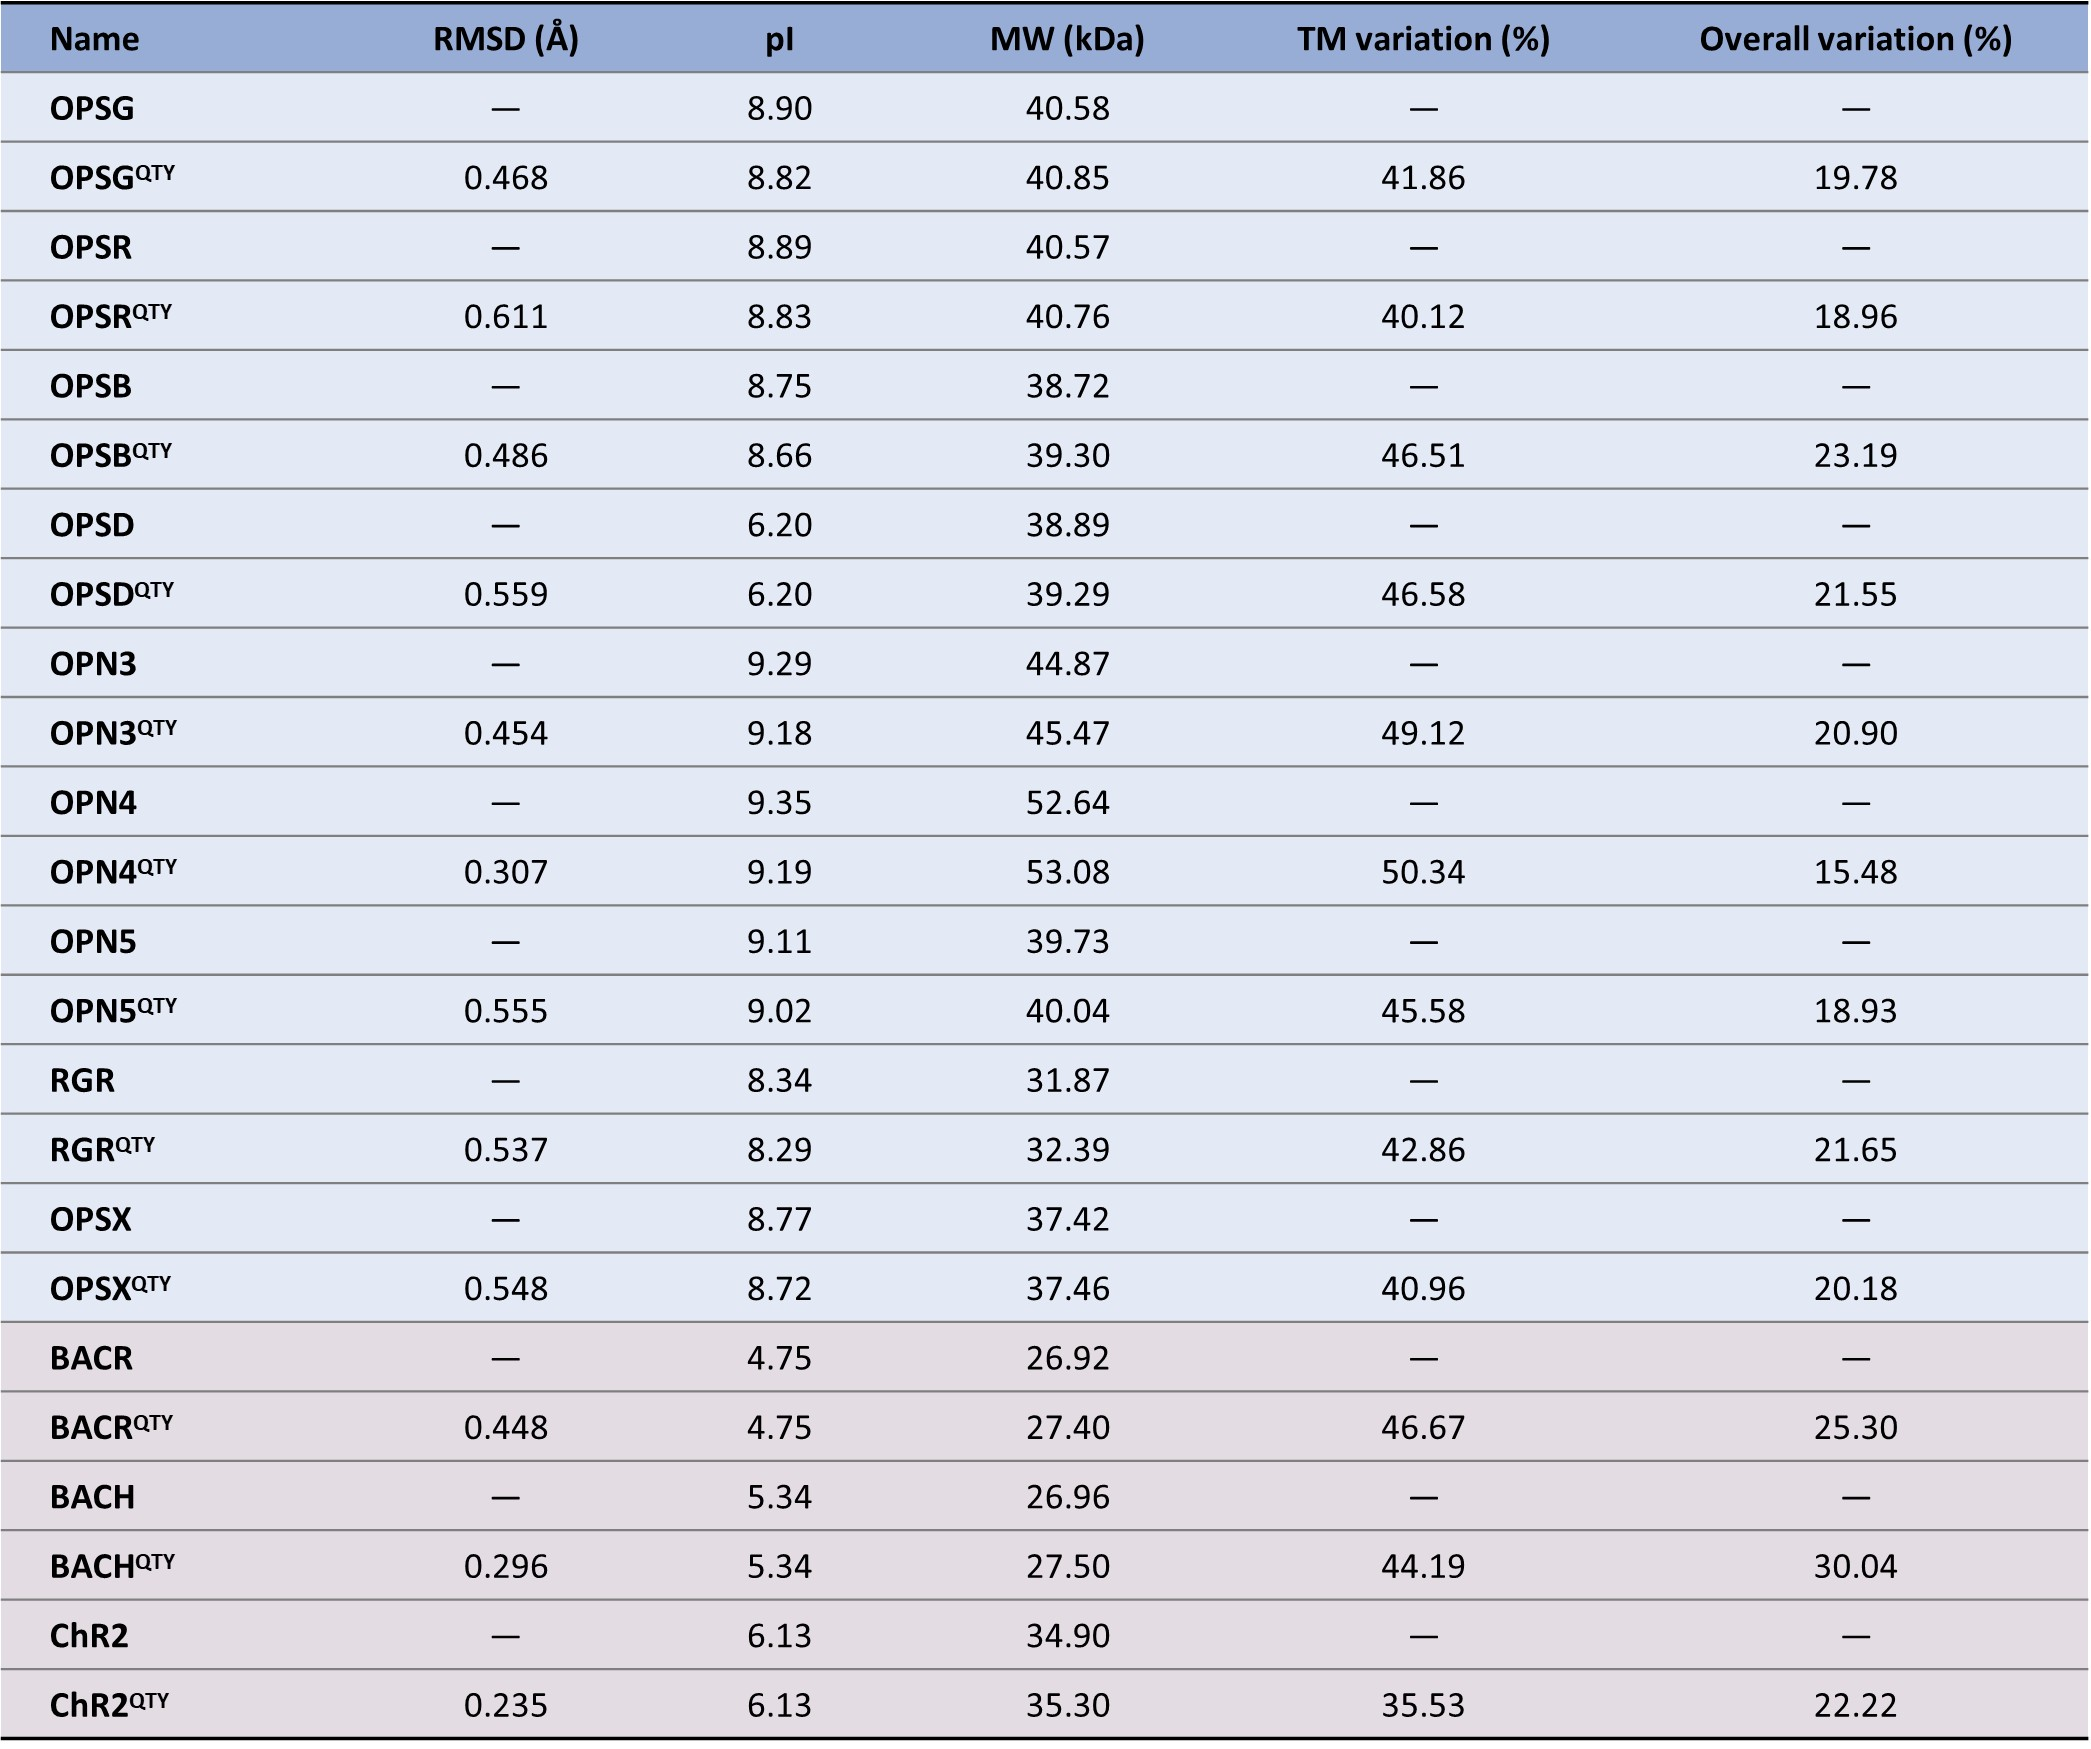
\includegraphics[width=\linewidth]{Figures/characteristics.jpg}
\end{table}


\begin{figure}[htbp]
	\centering
	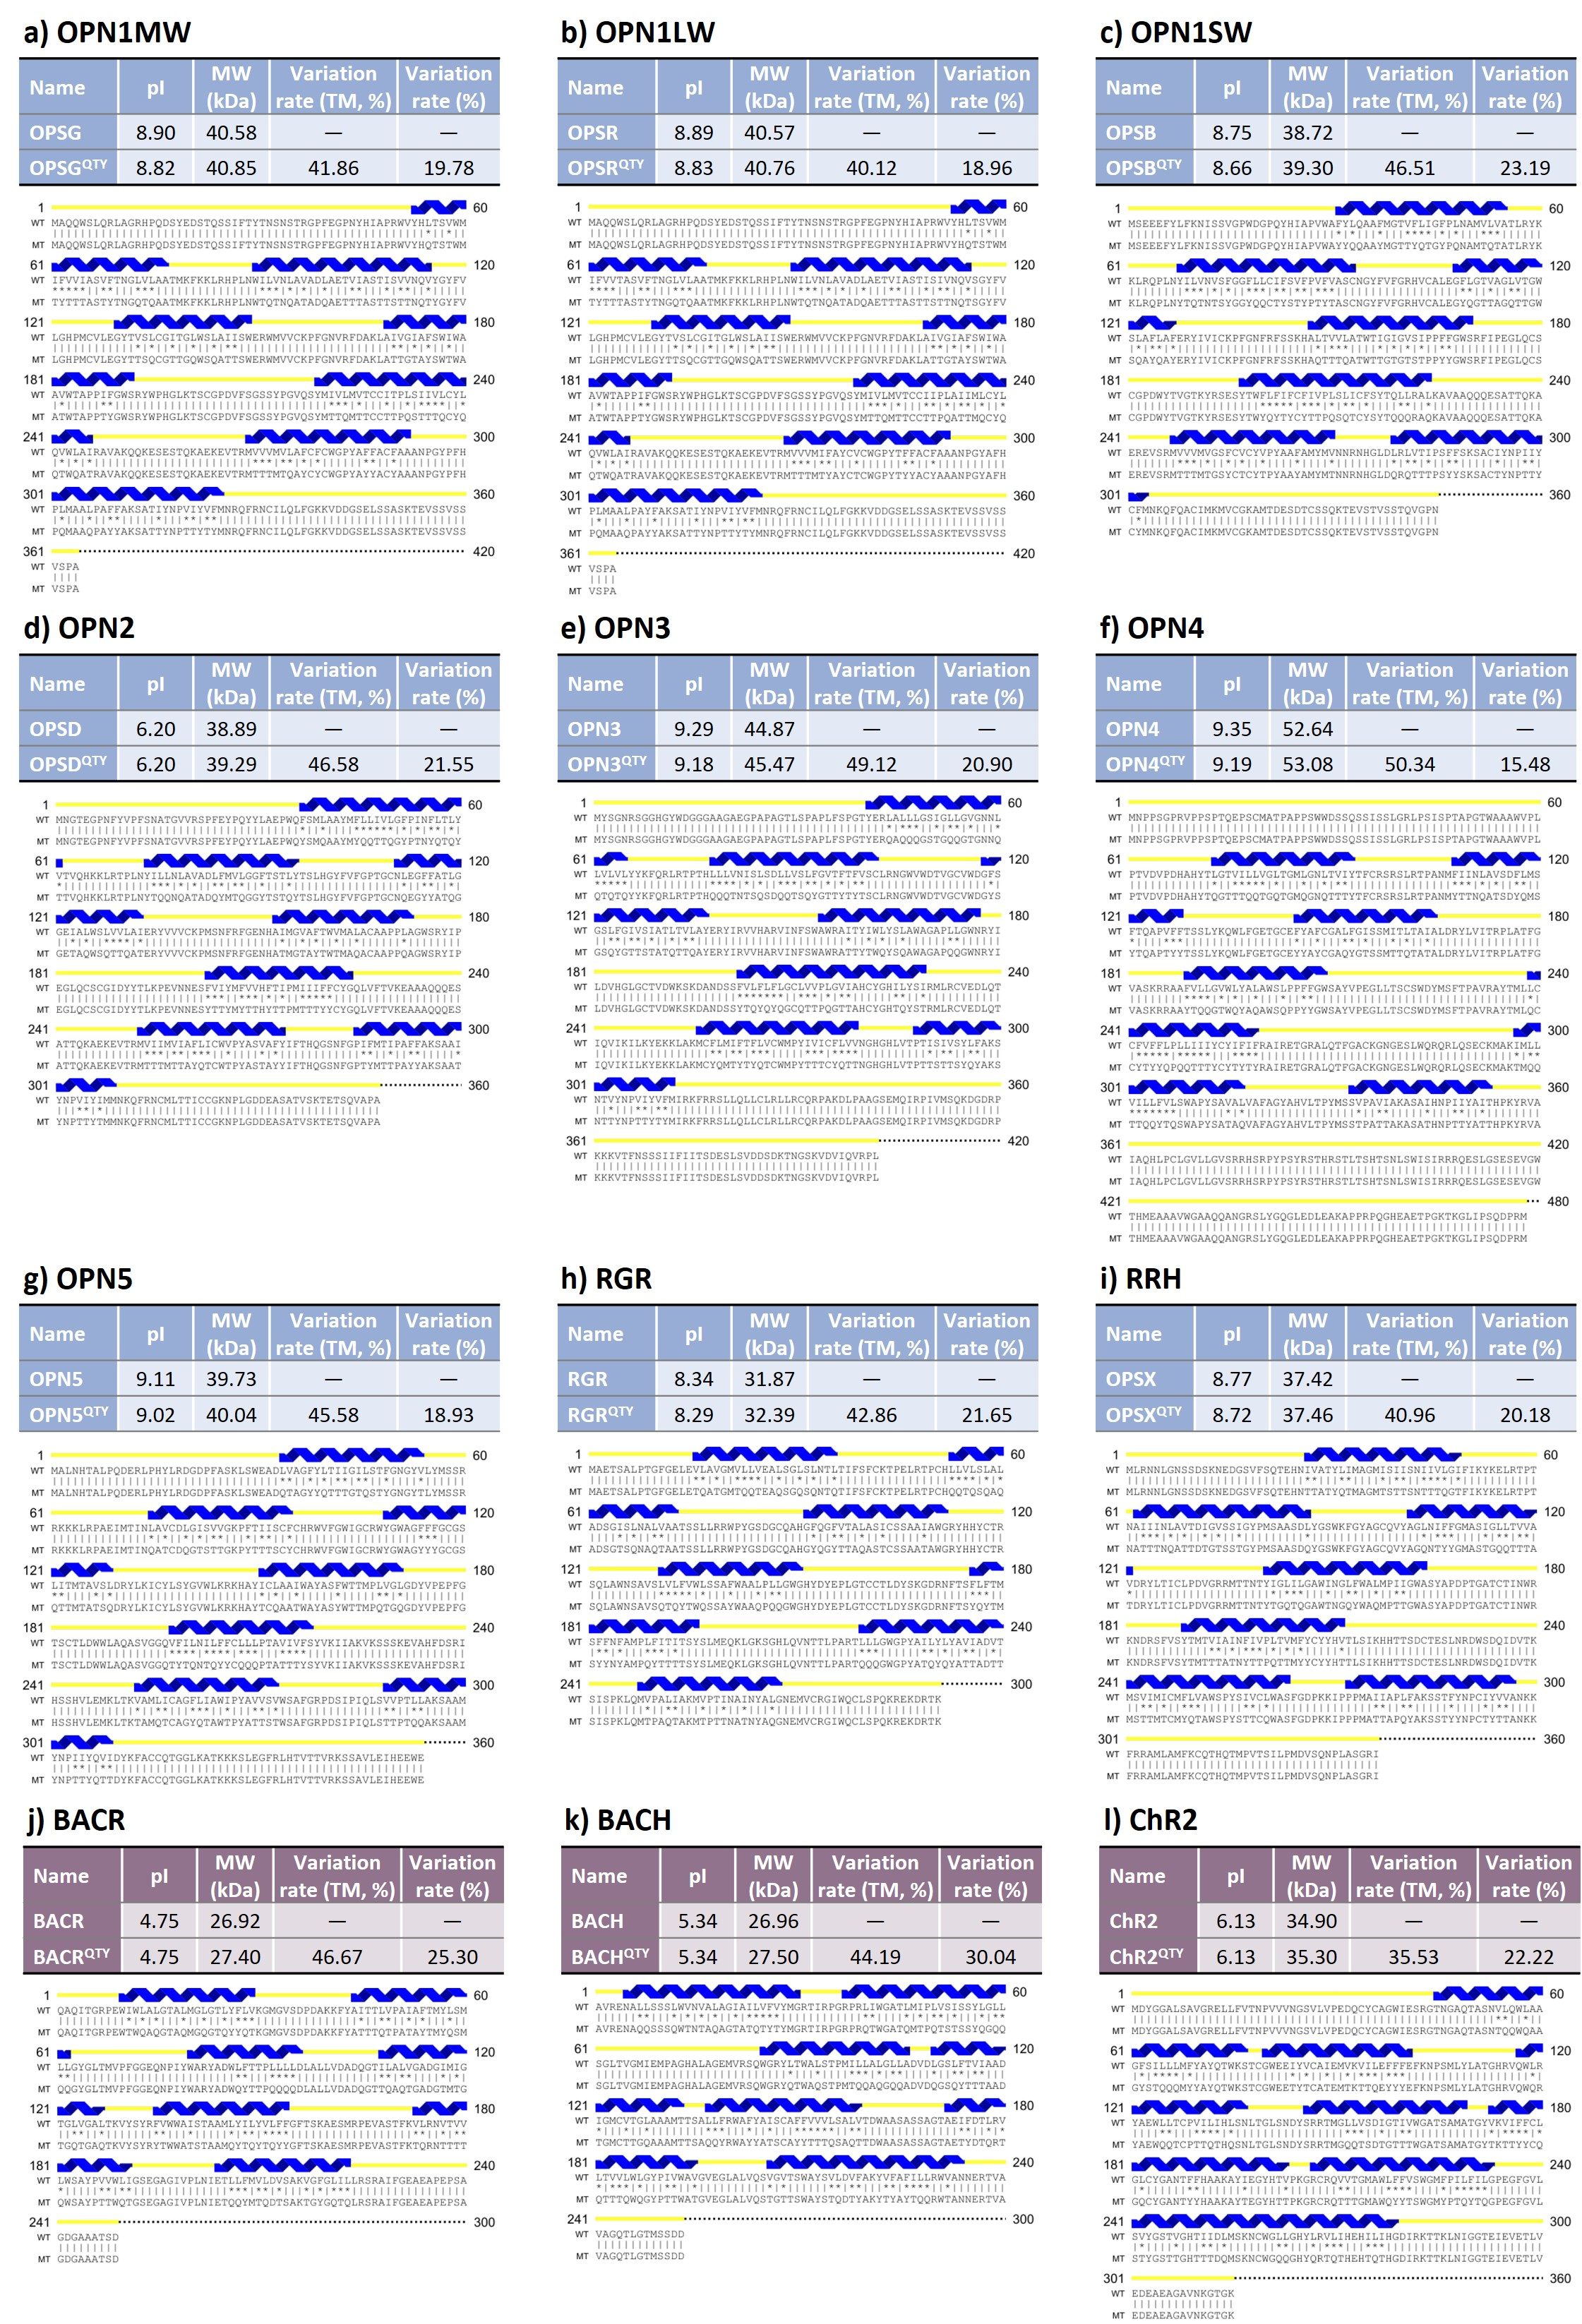
\includegraphics[width=\linewidth]{Figures/sequences.jpg}
	\caption{Protein sequence alignments}
	\label{fig:sequences}
\end{figure}

\begin{figure}[htbp]
	\centering
	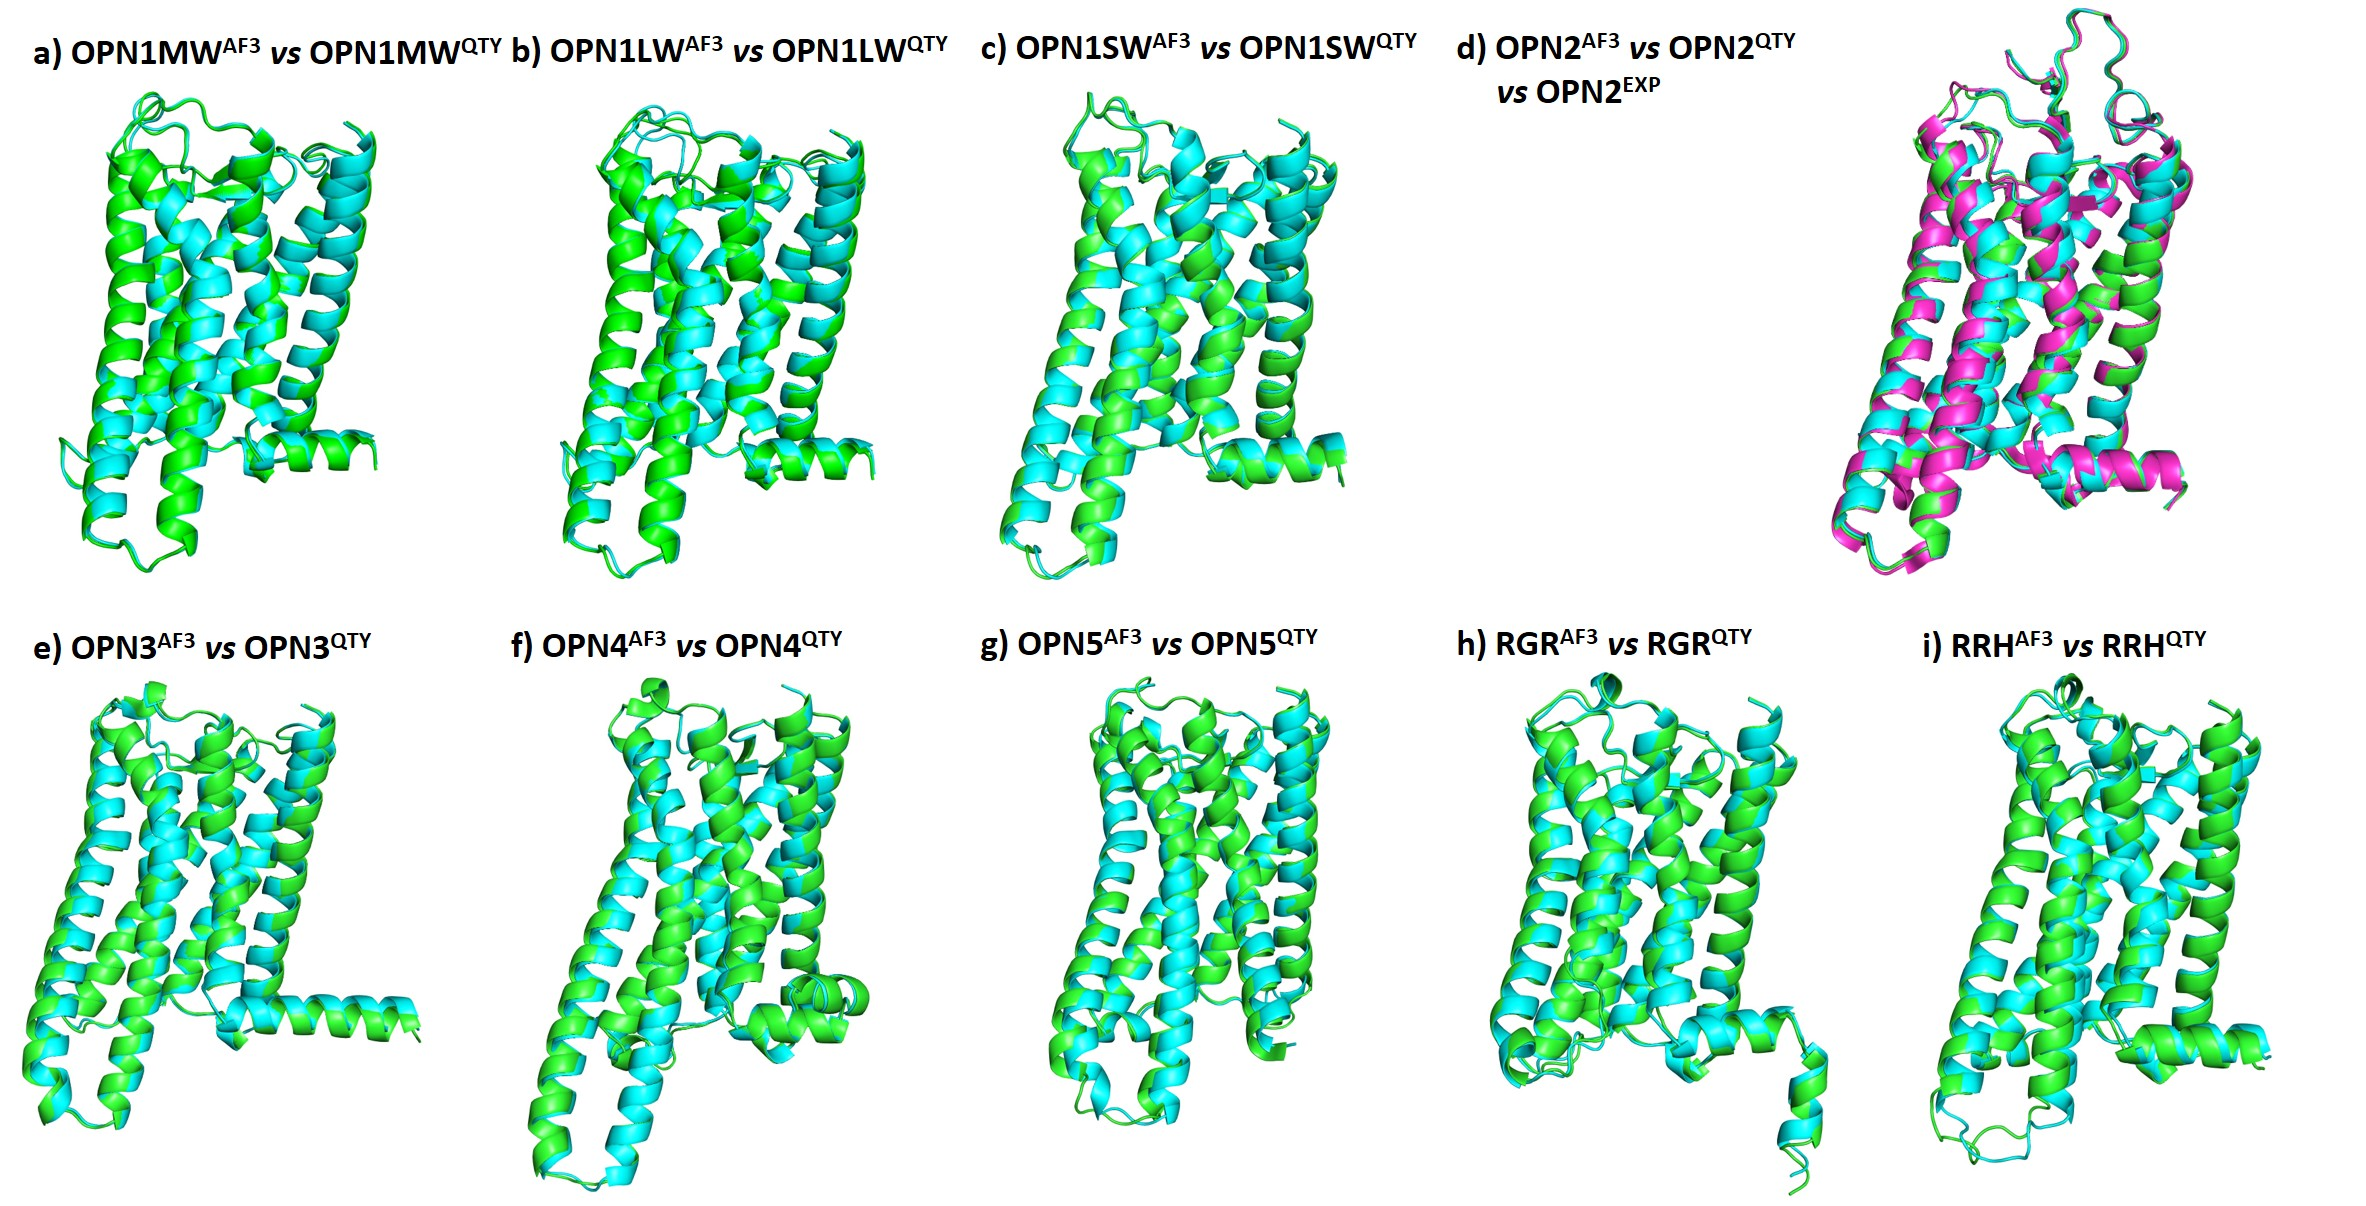
\includegraphics[width=\linewidth]{Figures/superposition-human.jpg}
	\caption{Superposition of human retinylidene proteins}
	\label{fig:humansup}
\end{figure}

\begin{figure}[htbp]
	\centering
	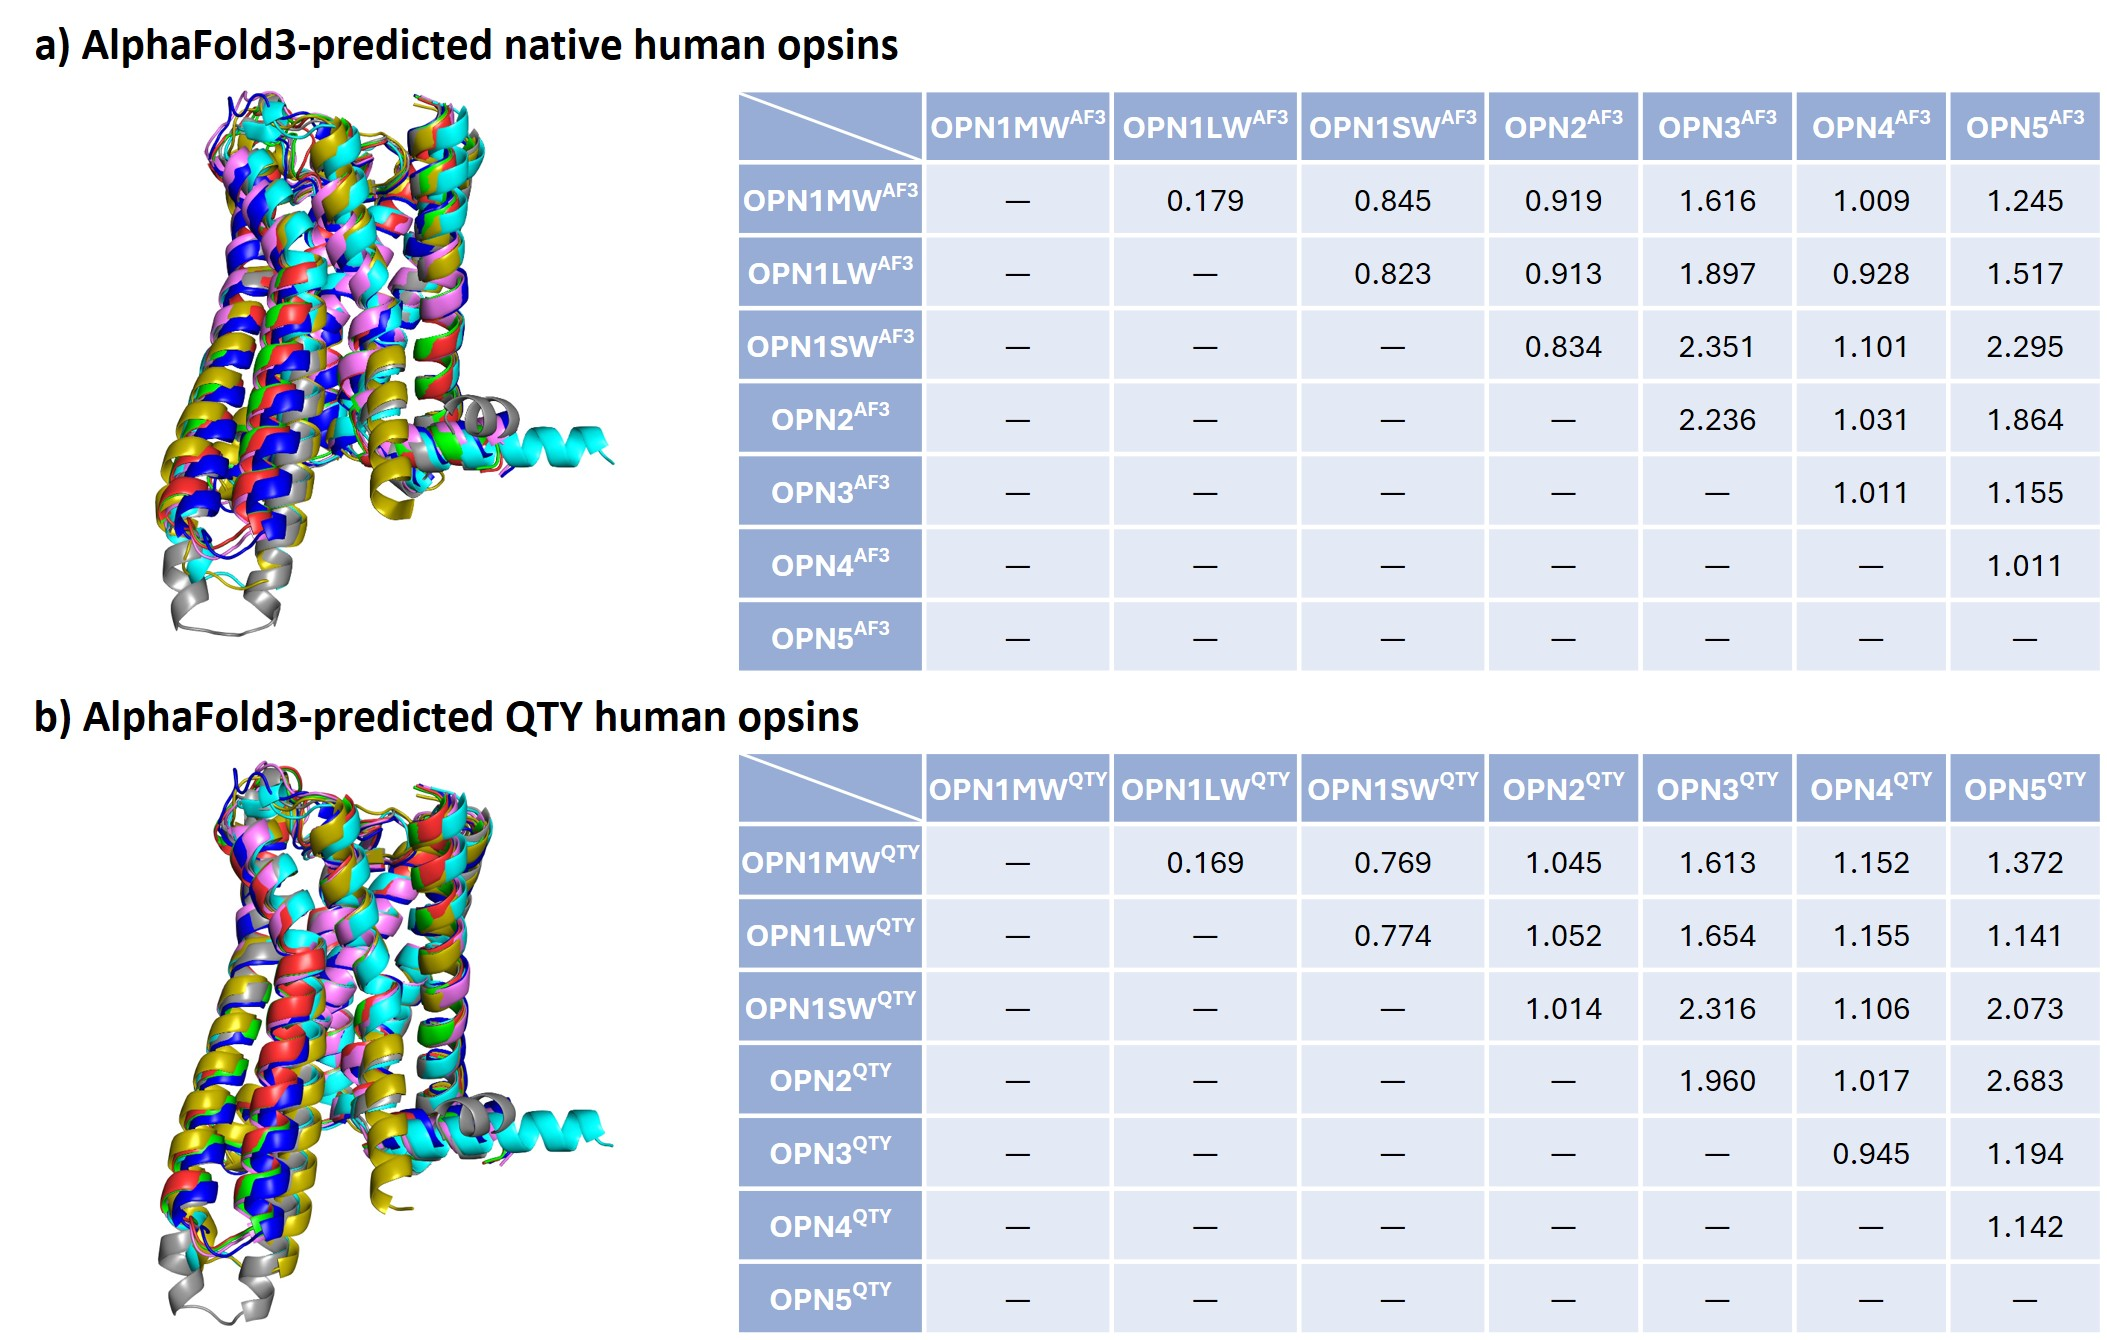
\includegraphics[width=\linewidth]{Figures/pairwise.jpg}
	\caption{Pairwise comparison of human opsins. Green: OPN1MW; red: OPN1LW; blue: OPN1SW; purple: OPN2; cyan: OPN3; gray: OPN4; olive: OPN5; orange: RGR; pink: RRH. }
	\label{fig:pairwise}
\end{figure}

\begin{figure}[htbp]
	\centering
	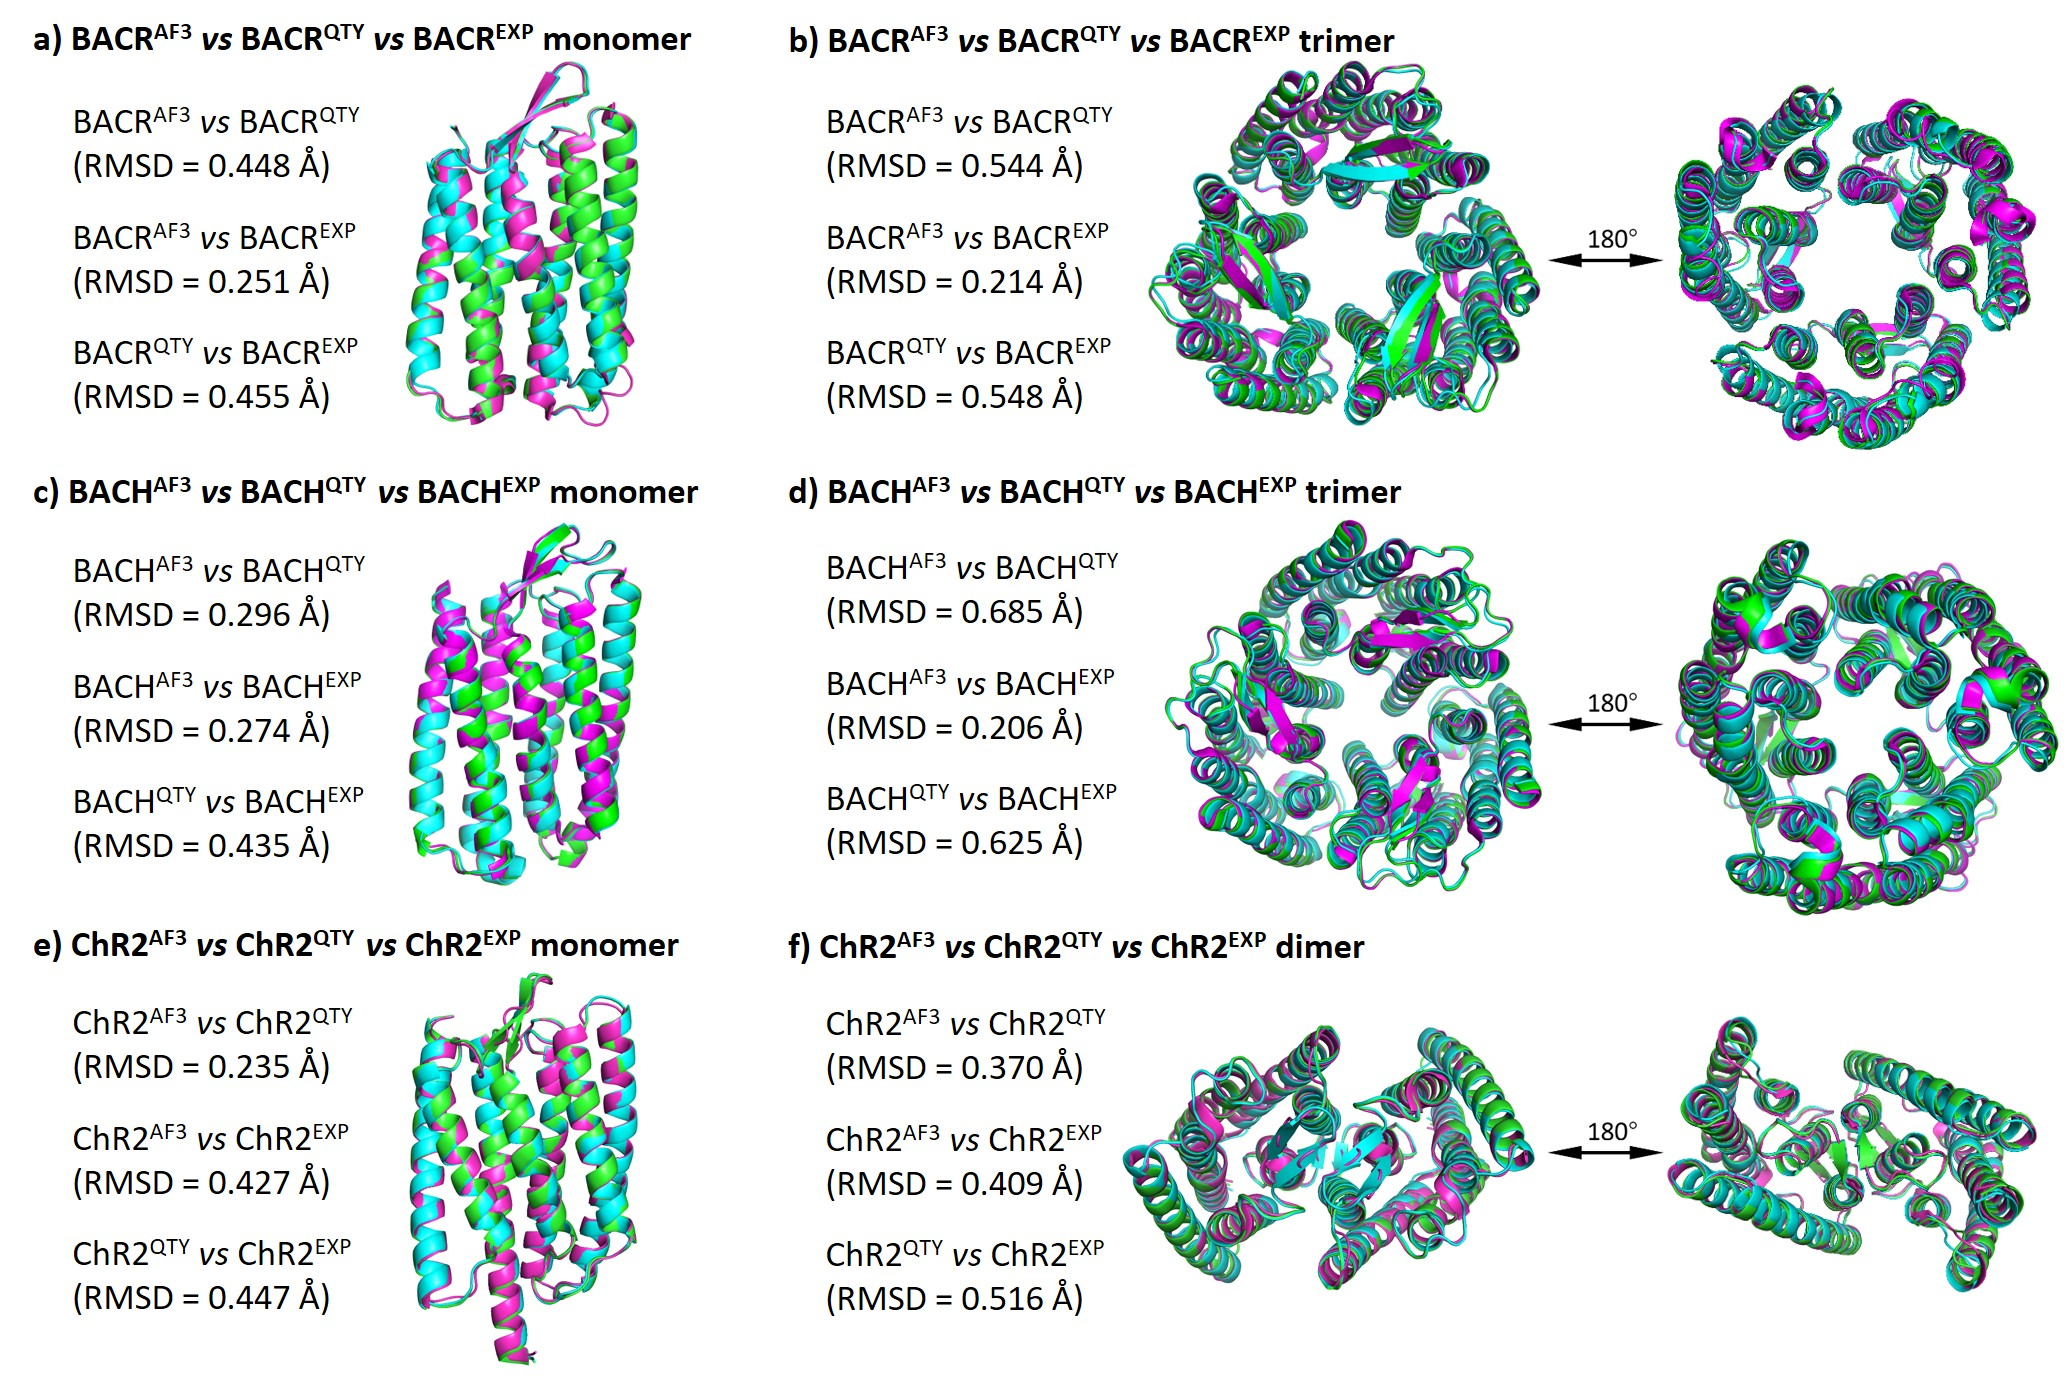
\includegraphics[width=\linewidth]{Figures/superposition-microbial.jpg}
	\caption{Superposition of microbial retinylidene proteins}
	\label{fig:microbialsup}
\end{figure}

\begin{figure}[htbp]
	\centering
	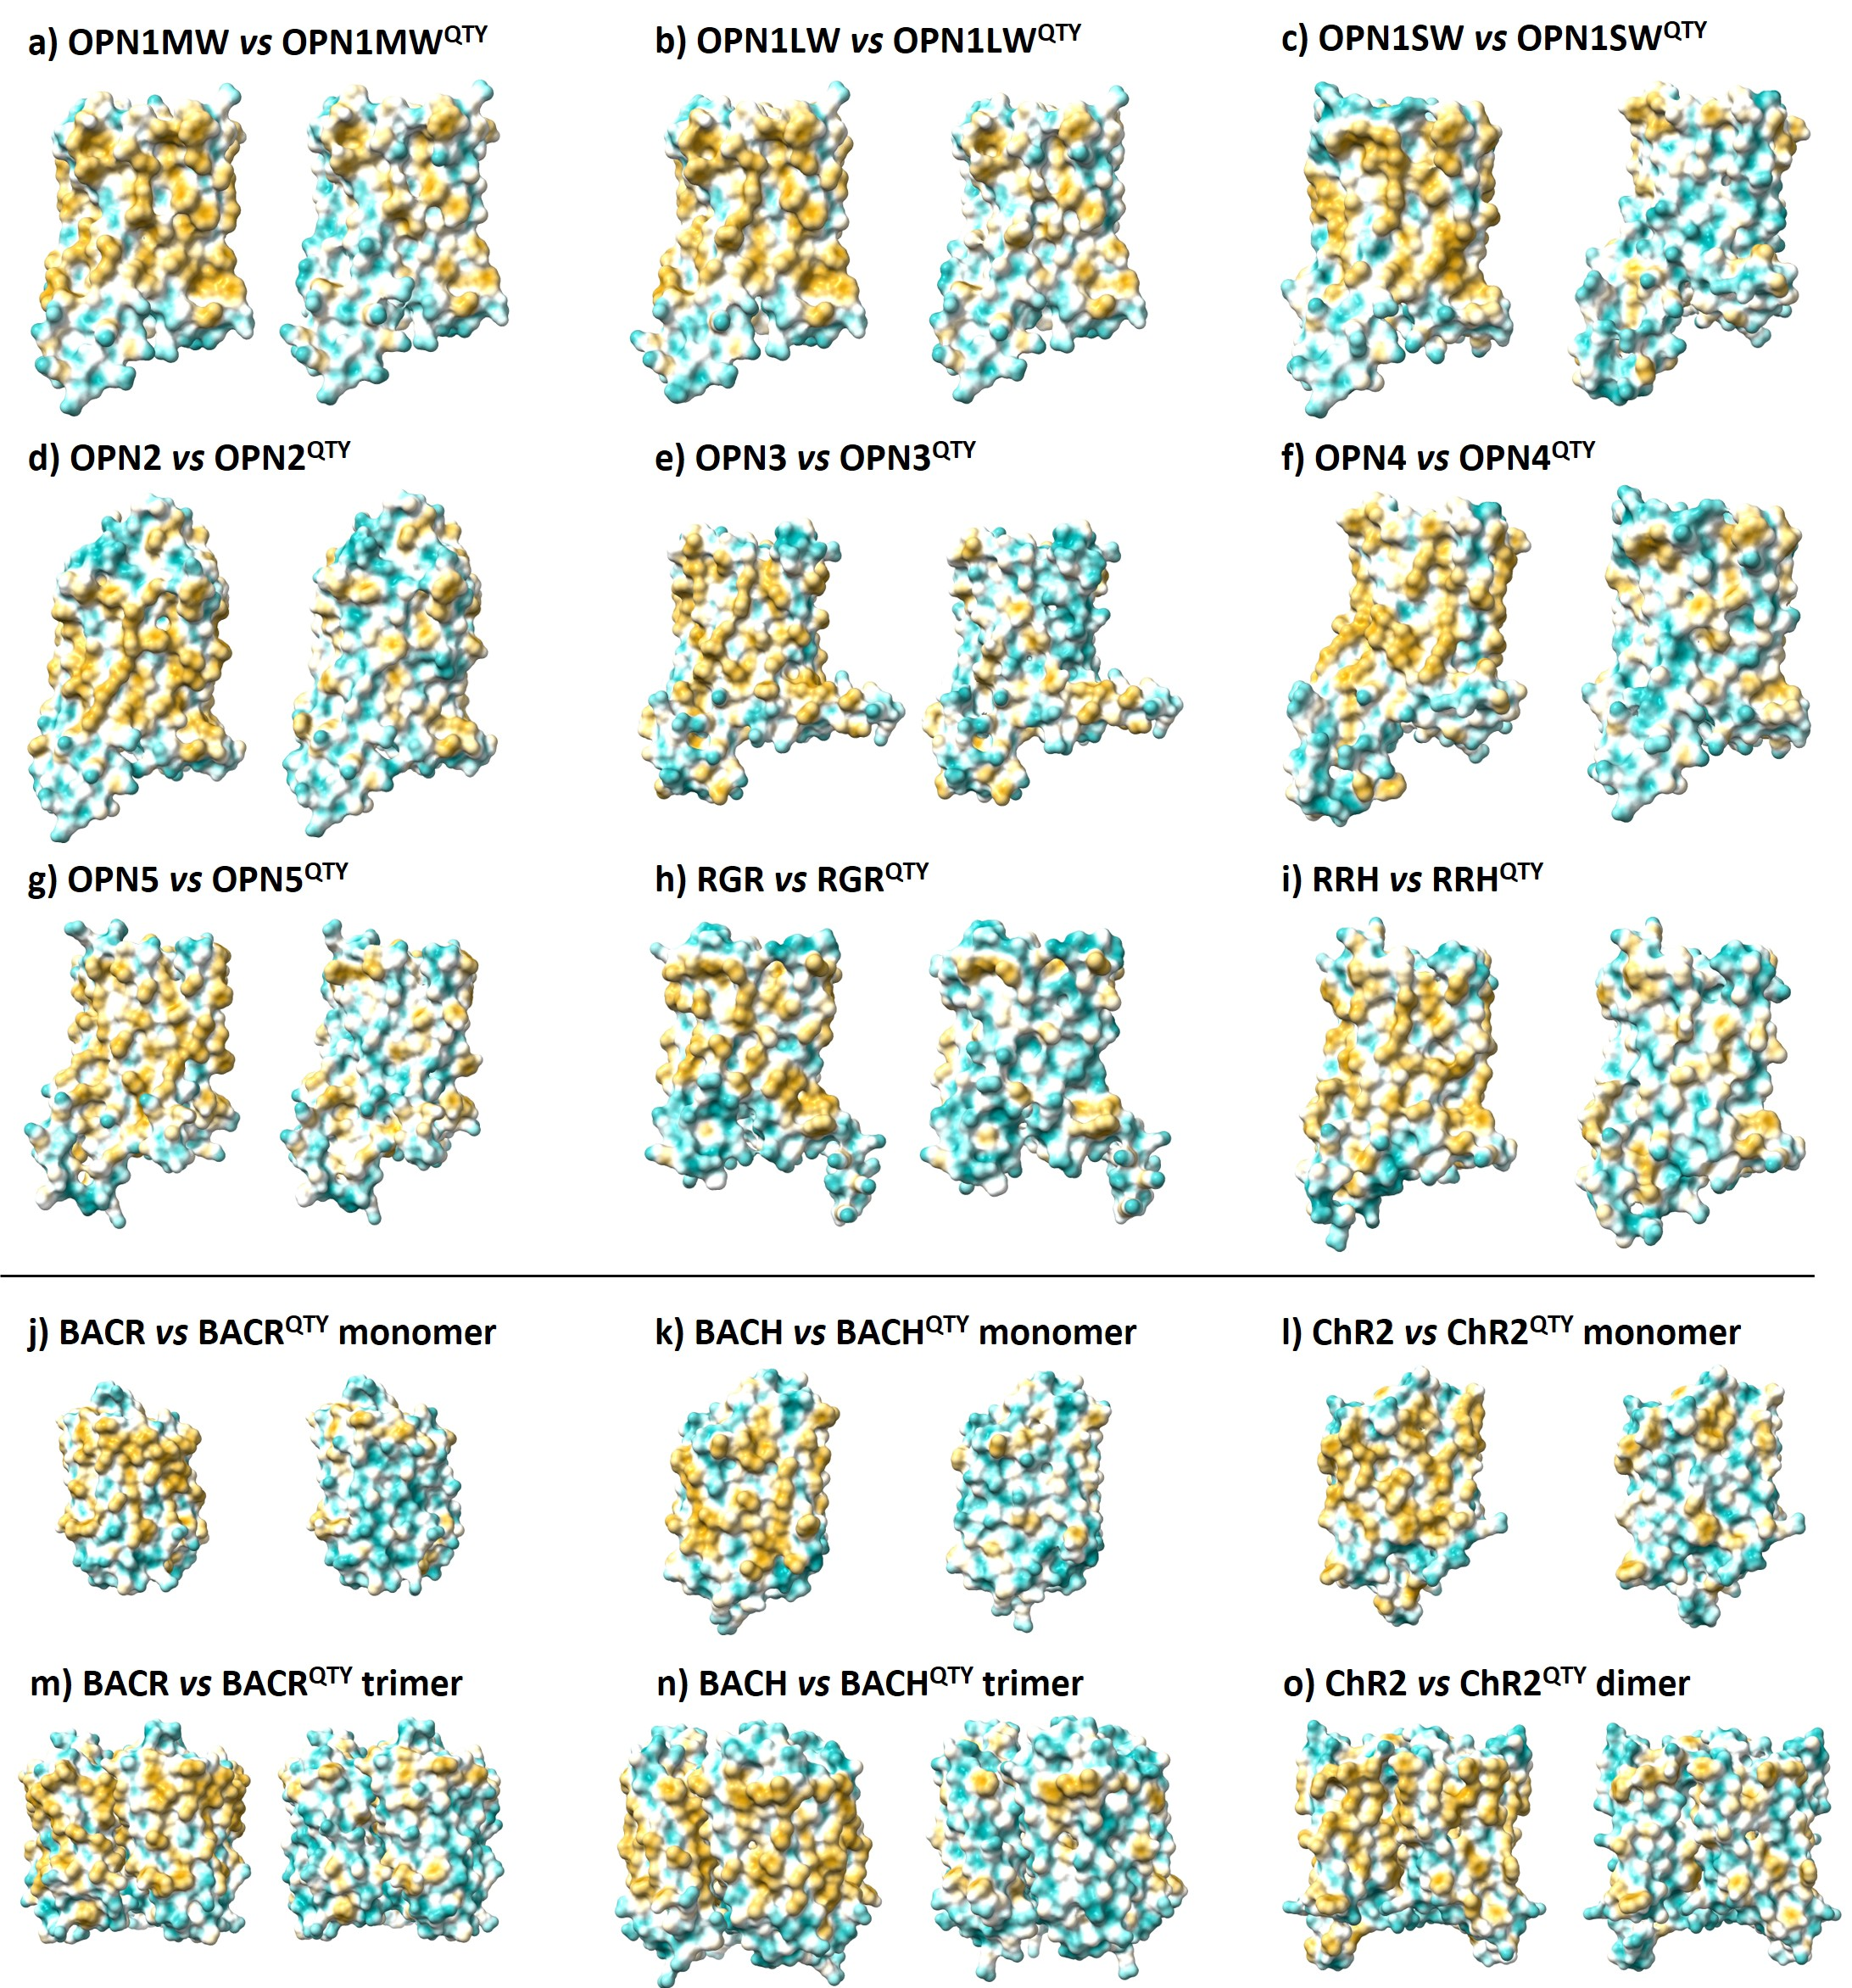
\includegraphics[width=\linewidth]{Figures/hydrophobicity.jpg}
	\caption{Surface hydrophobicity}
	\label{fig:hydrophobicity}
\end{figure}

\end{document}